\documentclass[journal]{IEEEtran}

\usepackage{amsmath,amssymb,amsfonts}
\usepackage{graphicx}
\usepackage{booktabs}
\usepackage{tabularx}
\usepackage{multirow}
\usepackage{cite}
\usepackage{url}
\usepackage{xcolor}
\usepackage{tikz}
\usetikzlibrary{arrows.meta,positioning,fit,calc}
\usepackage{algorithm}
\usepackage{algorithmic}
\usepackage{balance}
\usepackage{subcaption}

\begin{document}

\title{Confidence-Gated Multi-Agent Fall Detection: Retrieval-Augmented Reasoning and Cost-Sensitive Response on Wearable IMU Data}

\author{%
\IEEEauthorblockN{Anonymous Authors}
\IEEEauthorblockA{%
\textit{Anonymous Institution}\\
Email: anonymous@example.com}
}

\maketitle

\begin{abstract}
Wearable inertial fall detectors achieve strong average accuracy but remain brittle on ambiguous near-fall activities and provide neither calibrated uncertainty routing nor an explicit response policy under asymmetric false-negative cost. We present a \emph{Risk-Calibrated Dual-Process} (RCDP) architecture---a confidence-gated multi-agent wrapper around a fixed Tier-1 detector (CNN--LSTM--Attention following Bhatti \textit{et al.})---with (i)~a dual-threshold confidence gate, (ii)~retrieval-augmented $k$-nearest-neighbor case memory, (iii)~local large-language-model (LLM) chain-of-thought reasoning over biomechanical evidence, and (iv)~a cost-sensitive action agent. On an \emph{ambiguous stress benchmark} (SisFall D18/D19 near-falls, $n{=}300$/fold), Tier-1 F1 collapses from $0.713$ to $0.896$ with the full stack ($\Delta\text{F1}{=}+0.183$, $\Delta\text{Recall}{=}+0.208$, $84\%$ cost reduction). Under subject-independent five-fold cross-validation on the main protocol ($n{=}1000$/fold), mean F1 improves from $0.759{\pm}0.014$ to $0.887{\pm}0.029$ and recall from $0.759{\pm}0.022$ to $0.977{\pm}0.037$, with normalized response cost reduced by approximately $83\%$. External validation on binary KFall confirms cross-domain stability (F1 $0.987{\rightarrow}0.990$) rather than large headline gains. Paired ambiguous-case comparisons show Mistral substantially outperforms a heuristic reasoner (mean F1 $0.972$ vs.\ $0.034$). We position results as gains over a fair reimplementation of the Bhatti-style detector under our protocol, not as a claim against the original KFall multi-phase tables.
\end{abstract}

\begin{IEEEkeywords}
Fall detection, wearable IMU, confidence gating, retrieval-augmented reasoning, large language models, cost-sensitive decision making, SisFall, selective prediction.
\end{IEEEkeywords}

\section{Introduction}
\label{sec:intro}

Population aging and independent living motivate continuous fall monitoring with wearable inertial measurement units (IMUs)~\cite{iglesias2019wearable,nurek2020fallsurvey,khan2017review,sisfall2017}. Modern deep detectors can reach competitive accuracy on curated benchmarks~\cite{ren2021survey}, yet practical systems still fail in three ways that matter for safety-critical deployment. First, near-fall activities (e.g., sitting with compensatory motions) induce ambiguous windows that a softmax classifier force-labels~\cite{aziz2016fall}. Second, edge models rarely expose calibrated uncertainty that can defer difficult cases~\cite{guo2017calibration,geifman2017selective,el2010foundations}. Third, a binary fall/ADL prediction is not a response policy: emergency escalation, caregiver notification, and logging have unequal costs, especially when false negatives dominate clinical risk~\cite{elkan2001foundations}.

Bhatti \textit{et al.}~\cite{bhatti2025beyond} propose a strong hybrid CNN--LSTM--Attention detector for multi-phase fall analysis on wearable IMUs (``Beyond Falls''). Their contribution is primarily \emph{detection}. We ask a complementary question: \emph{given a fixed Tier-1 detector, can an agentic wrapper improve the safety operating point---raising recall and lowering expected response cost---while providing structured explanations on escalated windows?}

This paper answers affirmatively with an RCDP pipeline: a fast \emph{System~1} edge reflex (Tier-1 detector, $\approx 7$\,ms) routes confident windows deterministically, while ambiguous windows escalate to a deliberative \emph{System~2} (evidence serialization, $k$-NN memory, local LLM CoT, cost-sensitive Action Agent). Uncertain predictions are escalated to an evidence serializer, a growing $k$-NN memory of past cases, and a local LLM reasoner that emits JSON rationales~\cite{wei2022cot,lewis2020rag,yao2023react}; an Action Agent then maps decisions to simulated response tiers under asymmetric clinical cost $\mathcal{R}_\beta=\beta\cdot\mathrm{FN}+\mathrm{FP}$ with $\beta{=}10$. Our primary evaluation is SisFall~\cite{sisfall2017} with subject-independent five-fold cross-validation, forced inclusion of near-fall codes D18/D19, and a homogeneous evaluation budget of $1000$ stratified windows per fold. We additionally report an ambiguous stress benchmark ($n{=}300$/fold), larger-budget archives ($n{=}4000$), multi-seed training variability, latency profiles, and completed binary KFall external validation~\cite{kfall2021}.

\paragraph{Contributions.}
\begin{itemize}
\item A complete agentic architecture---gate, evidence, retrieval, LLM CoT, action---wrapped around a Bhatti-style Tier-1 backbone without modifying its weights at inference.
\item A locked paper protocol (splits, calibration, cost, near-fall metrics) that enables fair ablations: \texttt{tier1\_only} $\rightarrow$ \texttt{gate\_only} $\rightarrow$ \texttt{gate\_knn} $\rightarrow$ \texttt{gate\_llm} $\rightarrow$ \texttt{gate\_knn\_llm}.
\item Five-fold SisFall evidence that the full stack improves F1/recall and normalized cost on every fold, with an \textbf{ambiguous stress benchmark} (D18/D19) where Tier-1 F1 is $0.713$ vs.\ $0.896$ for the stack ($\Delta\text{F1}{=}+0.183$).
\item Paired LLM backend comparisons on shared ambiguous IDs, budget-sensitivity figures, binary KFall external validation, and latency characterization of the escalated path.
\item An honest positioning relative to Bhatti~\textit{et al.}: gains are versus the \emph{same} Tier-1 checkpoint under our SisFall protocol; we do not claim to supersede the original KFall multi-phase tables.
\end{itemize}

\section{Related Work}
\label{sec:related}

\subsection{Wearable Fall Detection}
Classical threshold detectors~\cite{bourke2007threshold} and shallow learners have been succeeded by CNN, LSTM, TCN, and Transformer variants on public corpora such as SisFall~\cite{sisfall2017}, KFall~\cite{kfall2021}, UP-Fall~\cite{martinez2019upfall}, and UniMiB SHAR~\cite{micucci2017unimib}. Surveys emphasize the trade-off between sensitivity and false alarms in free living~\cite{iglesias2019wearable,khan2017review,ren2021survey}. Bhatti \textit{et al.}~\cite{bhatti2025beyond} integrate CNN, LSTM, and attention for pre-/transition-/post-fall phases on KFall. We reuse their architectural motif as Tier-1 and add decision-time agents rather than proposing another detector backbone as the sole contribution.

\subsection{Uncertainty, Calibration, and Selective Prediction}
Modern networks are often miscalibrated~\cite{guo2017calibration,platt1999probabilistic}. Selective classification and abstention~\cite{el2010foundations,geifman2017selective} motivate routing low-confidence samples to stronger (or human) decision makers. Our dual-threshold gate implements selective escalation tailored to fall cost asymmetry, rather than a single reject option.

\subsection{Retrieval-Augmented and Agentic LLM Reasoning}
Retrieval-augmented generation~\cite{lewis2020rag} and compact encoders such as MiniLM~\cite{minilm2020} support case-based reasoning. Chain-of-thought prompting~\cite{wei2022cot} and reason--act loops~\cite{yao2023react} improve structured decisions. Local LLM runtimes~\cite{ollama,mistral2023,qwen2024} enable offline CoT without cloud APIs. We apply these ideas to IMU-derived biomechanical evidence rather than text-native tasks, and we close the loop with a cost-sensitive Action Agent.

\section{Method}
\label{sec:method}

Fig.~\ref{fig:arch} summarizes the pipeline.

\begin{figure*}[!t]
\centering
% TikZ architecture figure for agentic fall detection pipeline
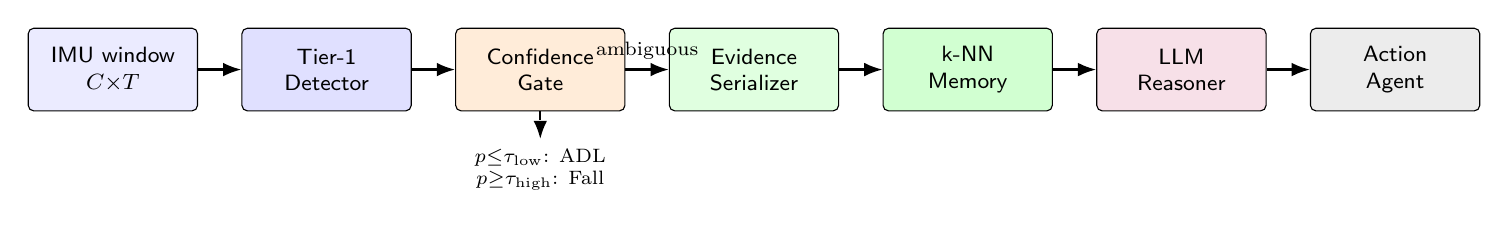
\begin{tikzpicture}[
  font=\footnotesize,
  box/.style={draw, rounded corners=2pt, align=center, inner sep=4pt, minimum height=1.05cm, minimum width=2.15cm},
  arr/.style={-{Latex}, thick},
  every node/.style={font=\footnotesize\sffamily}
]
\node[box, fill=blue!8] (imu) {IMU window\\$C{\times}T$};
\node[box, fill=blue!12, right=0.55cm of imu] (tier1) {Tier-1\\Detector};
\node[box, fill=orange!15, right=0.55cm of tier1] (gate) {Confidence\\Gate};
\node[box, fill=green!12, right=0.55cm of gate] (ev) {Evidence\\Serializer};
\node[box, fill=green!18, right=0.55cm of ev] (knn) {k-NN\\Memory};
\node[box, fill=purple!12, right=0.55cm of knn] (llm) {LLM\\Reasoner};
\node[box, fill=gray!15, right=0.55cm of llm] (act) {Action\\Agent};

\draw[arr] (imu) -- (tier1);
\draw[arr] (tier1) -- (gate);
\draw[arr] (gate) -- node[above, font=\scriptsize] {ambiguous} (ev);
\draw[arr] (ev) -- (knn);
\draw[arr] (knn) -- (llm);
\draw[arr] (llm) -- (act);

\node[below=0.35cm of gate, font=\scriptsize, align=center] (direct) {$p{\le}\tau_{\mathrm{low}}$: ADL\\$p{\ge}\tau_{\mathrm{high}}$: Fall};
\draw[arr, dashed] (gate.south) -- (direct.north);
\end{tikzpicture}

\caption{Confidence-gated multi-agent fall detection. High/low confidence windows are decided by the Tier-1 detector; ambiguous windows escalate to evidence serialization, $k$-NN retrieval, LLM reasoning, and a cost-sensitive Action Agent.}
\label{fig:arch}
\end{figure*}

\subsection{Tier-1 Detector}
Given a window $\mathbf{x}\in\mathbb{R}^{C\times T}$ (here $C{=}6$, $T{=}90$ on SisFall), a backbone $f_\theta$ produces logits and embedding $\mathbf{e}$. We convert logits to fall probability $p(\mathrm{fall})$. The primary backbone is CNN--LSTM--Attention following Bhatti~\textit{et al.}~\cite{bhatti2025beyond}; we additionally train a zoo (CNN1D, LSTM, CNN--LSTM, TCN, ModernTCN~\cite{iglesias2023modern}, TSMixer~\cite{tsmixer2023}, PatchTST~\cite{patchtst2023}, Transformer~\cite{vaswani2017attention}) under the same protocol for context (Table~\ref{tab:backbone}).

\subsection{Confidence Gate}
A dual-threshold gate with calibrated $(\tau_{\mathrm{low}},\tau_{\mathrm{high}})$ routes windows:
\begin{equation}
\begin{cases}
\mathrm{ADL}, & p \le \tau_{\mathrm{low}},\\
\mathrm{Fall}, & p \ge \tau_{\mathrm{high}},\\
\mathrm{Ambiguous}, & \text{otherwise.}
\end{cases}
\end{equation}
Thresholds are calibrated on subject-held-out training windows. Mode \texttt{tier1\_only} disables meaningful escalation by collapsing the ambiguous band to a point decision at $0.5$.

\subsection{Evidence Serializer}
For escalated windows we compute biomechanical descriptors (free-fall duration, impact magnitude, post-impact stillness, tilt change, peak gyroscope) and serialize them into natural-language evidence for retrieval and prompting.

\subsection{Retrieval Memory}
A $k$-NN memory stores MiniLM~\cite{minilm2020} embeddings of evidence text with labels and features. At escalation time we retrieve $k{=}5$ neighbors (cosine similarity) as few-shot context, following the RAG principle~\cite{lewis2020rag}.

\subsection{LLM Reasoner}
An LLM reasoner (backend $\in\{\texttt{ollama},\texttt{heuristic}\}$) consumes evidence and neighbors and returns a JSON decision with rationale~\cite{wei2022cot}. We evaluate heuristic, Mistral~\cite{mistral2023}, and Qwen2.5~\cite{qwen2024} on paired ambiguous IDs. Production full-stack rows use Ollama~\cite{ollama} with Mistral as the default local model.

\subsection{Action Agent and Cost}
The Action Agent maps severity cues to simulated actions (emergency / notify / monitor / log). Expected response cost uses
\begin{equation}
\mathrm{Cost} = 10\cdot \mathrm{FN} + 1\cdot \mathrm{FP}.
\end{equation}
We report \emph{cost per 1000 windows} so folds with equal evaluation budgets are comparable. The FN weight encodes the clinical preference that missed falls are substantially more expensive than false alarms~\cite{elkan2001foundations}.

\subsection{System Modes}
Ablations instantiate cumulative agents:
\texttt{tier1\_only}, \texttt{gate\_only}, \texttt{gate\_knn}, \texttt{gate\_llm}, and \texttt{gate\_knn\_llm} (full stack). The design isolates whether gains require retrieval, language-model reasoning, or both.


\subsection{Deployment Workflow}
\label{sec:deployment}
Fig.~\ref{fig:deployment} illustrates the RCDP dual-process deployment model. \emph{System~1} executes on-device reflex classification ($\approx 7$\,ms per window): confident ADL and fall decisions are logged or alarmed without cloud invocation. Ambiguous windows escalate to \emph{System~2}, which operates during the post-impact immobility window ($\approx 10$--$60$\,s) using biomechanical evidence $\Sigma(w)$, retrieval-augmented reasoning, and optional contrastive critique before emitting a graded action policy. Table~\ref{tab:escalation} reports honest escalation duty cycles by protocol.

\begin{figure*}[!t]
\centering
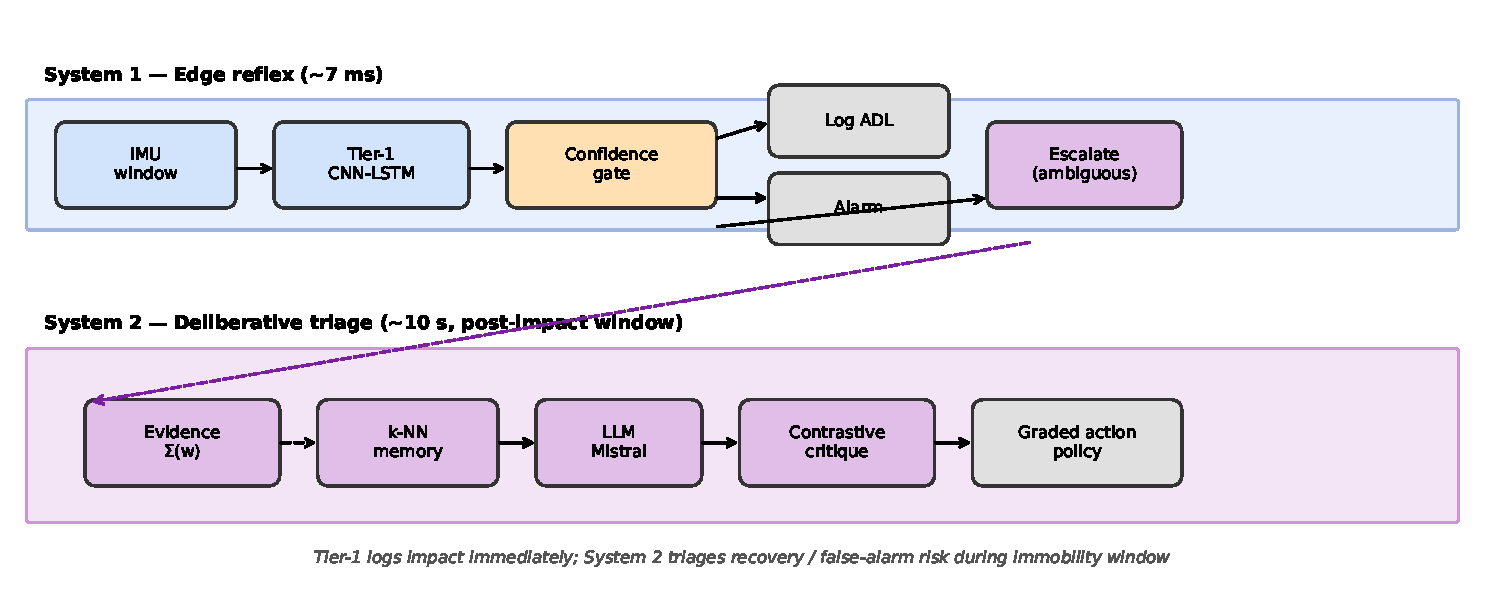
\includegraphics[width=\linewidth]{fig/deployment_architecture.pdf}
\caption{RCDP deployment workflow: System~1 edge reflex (milliseconds) vs.\ System~2 deliberative triage (seconds) on escalated ambiguous windows.}
\label{fig:deployment}
\end{figure*}

\begin{table}[!t]
\centering
\caption{System~2 escalation duty cycle by evaluation protocol (honest reporting). High rates on the ambiguous stress benchmark reflect deliberate near-fall stress; KFall external transfer invokes deliberation on $\approx$1\% of windows.}
\label{tab:escalation}
\begin{tabular}{lcc}
\toprule
Protocol & $n$/fold & Escalation rate \\
\midrule
SisFall main (5-fold mean) & 1000 & 0.47 ($\pm$0.08) \\
SisFall ambiguous stress & 300 & 0.59 \\
KFall external (5-fold mean) & 1000 & 0.011 \\
\bottomrule
\end{tabular}
\end{table}


\subsection{Clinical Cost Framing and Grounding}
\label{sec:clinical}
Asymmetric clinical risk $\mathcal{R}_\beta=\beta\cdot\mathrm{FN}+\mathrm{FP}$ with penalty ratio $\beta$ shifts the Bayes-optimal threshold to $\tau^*=1/(\beta+1)$ (Table~\ref{tab:betacost}). To verify that LLM rationales are tied to telemetry rather than hallucinated severity, we report kinematic faithfulness $\mathcal{G}_{\mathrm{faith}}$: the fraction of rationales citing $\Sigma(w)$ primitives (Table~\ref{tab:grounding}). Contrastive critique raises mean $\mathcal{G}_{\mathrm{faith}}$ from $0.436$ to $0.843$ while reducing graded action cost by $\approx 45\%$.

\begin{table}[!t]
\centering
\caption{Asymmetric clinical cost sensitivity across penalty ratio $\beta=c_{\mathrm{FN}}/c_{\mathrm{FP}}\in\{5,10,20\}$ (cost $=\beta\cdot\mathrm{FN}+\mathrm{FP}$, per 1000 windows). Bayes optimal threshold $\tau^*=1/(\beta+1)$ motivates asymmetric escalation.}
\label{tab:betacost}
\begin{tabular}{lcccc}
\toprule
$\beta$ & $\tau^*$ & Mode & Mean cost/1000 & $\Delta$ vs Tier-1 \\
\midrule
5 & 0.167 & tier1\_only & 628 & --- \\
5 & 0.167 & \textbf{gate\_knn\_llm} & \textbf{149} & \textbf{-479} \\
\addlinespace
10 & 0.091 & tier1\_only & 1151 & --- \\
10 & 0.091 & \textbf{gate\_knn\_llm} & \textbf{200} & \textbf{-951} \\
\addlinespace
20 & 0.048 & tier1\_only & 2197 & --- \\
20 & 0.048 & \textbf{gate\_knn\_llm} & \textbf{302} & \textbf{-1895} \\
\bottomrule
\end{tabular}
\end{table}

\begin{table}[!t]
\centering
\caption{Kinematic faithfulness $\mathcal{G}_{\mathrm{faith}}$ (rationale grounding rate): fraction of LLM rationales citing biomechanical evidence $\Sigma(w)$ (impact $g$, stillness, tilt). Contrastive critique nearly doubles grounding with $\approx$45\% graded action cost reduction.}
\label{tab:grounding}
\begin{tabular}{ccccc}
\toprule
Fold & Base $\mathcal{G}_{\mathrm{faith}}$ & +Contrastive & Graded cost base & Graded cost +Critique \\
\midrule
0 & 0.430 & 0.851 & 544 & 268 \\
1 & 0.340 & 0.749 & 901 & 599 \\
2 & 0.471 & 0.871 & 535 & 261 \\
3 & 0.482 & 0.874 & 428 & 216 \\
4 & 0.459 & 0.868 & 537 & 274 \\
\midrule
Mean & 0.436 & \textbf{0.843} & 589 & \textbf{324} \\
\bottomrule
\end{tabular}
\end{table}


\section{Experimental Setup}
\label{sec:setup}

\subsection{Dataset and Splits}
We use SisFall~\cite{sisfall2017} windows with six IMU channels (window $90$, hop $10$). Subject-independent five-fold splits hold out subjects; within each training fold a subject-held-out validation fraction tunes training and gate calibration. Near-fall activities D18/D19 are required and forced into capped test slices (minimum $80$ windows per code). Processed SisFall yields on the order of $1.55{\times}10^{6}$ windows across $38$ subjects; main tables evaluate a homogeneous stratified budget of $n{=}1000$ per fold for compute-tractable LLM escalation, with $n{=}4000$ archives for budget sensitivity.

\subsection{Protocol}
Training uses class imbalance handling (\texttt{pos\_weight}), mixup, and cost-sensitive decision thresholds. The \textbf{main paper tables} use $n{=}1000$ stratified test windows per fold. Archived runs with $n{=}4000$ provide a detailed ablation ladder including \texttt{gate\_llm}. The global training seed for the primary tables is $42$; we additionally report a multi-seed sweep on Fold~0 to quantify training variability. Primary agentic backend is local Ollama/Mistral.

\subsection{Metrics}
We report F1, recall/sensitivity, specificity, near-fall false-alarm rate on D18/D19, escalated-subset F1, escalation rate, normalized response cost, and latency (Tier-1 ms vs.\ escalated-path seconds). Significance uses paired bootstrap $95\%$ confidence intervals of mean fold-wise deltas; Wilcoxon signed-rank $p$-values are reported for completeness ($n{=}5$). With complete sign agreement across five folds, Wilcoxon $p$ bottoms at $0.0625$; we therefore emphasize bootstrap CIs that exclude zero for the primary claims.

\subsection{External Validation Path (KFall)}
KFall~\cite{kfall2021} is the dataset emphasized in the Beyond Falls multi-phase setting. We evaluate binary Fall/ADL windows under the same cost/gate protocol as SisFall (\texttt{configs/tier1\_kfall\_binary.yaml}, \texttt{scripts/run\_kfall\_external.py}). Five-fold external validation is complete: Tier-1 F1 $0.987{\pm}0.005$ vs.\ stack $0.990{\pm}0.004$ ($\Delta\text{F1}{=}+0.003$), confirming cross-domain stability rather than large F1 gains. Cost/1000 decreases from $50{\pm}35$ to $26{\pm}12$.

\section{Results}
\label{sec:results}

\begin{table*}[!t]
\centering
\caption{Positioning relative to Bhatti \textit{et al.} (base detector paper).}
\label{tab:positioning}
\begin{tabular}{lll}
\toprule
Aspect & Bhatti \textit{et al.}~2025~\cite{bhatti2025beyond} & This work \\
\midrule
Primary task & Multi-phase fall/ADL classification & Detection + uncertainty + explanation + response \\
Backbone & CNN--LSTM--Attention & Same primary backbone + modern zoo \\
Uncertainty & Softmax confidence only & Dual-threshold confidence gate ($\tau_{\mathrm{low}},\tau_{\mathrm{high}}$) \\
Explainability & Attention weights & Structured biomechanical evidence + CoT JSON \\
Case memory & None & Retrieval-augmented $k$-NN memory \\
Response policy & None & Cost-sensitive Action Agent \\
Primary dataset in original paper & KFall (multi-class) & SisFall binary + near-fall ADLs (D18/D19) \\
Fair baseline in our tables & --- & \texttt{tier1\_only} (same checkpoint/folds) \\
\bottomrule
\end{tabular}
\end{table*}


\subsection{Ambiguous Stress Benchmark (Lead Result)}
\label{sec:ambiguous}
Near-fall activities D18 (stumbling) and D19 (sudden sitting) are the primary failure mode of threshold and softmax classifiers. We therefore evaluate a dedicated \emph{ambiguous stress benchmark} with $n{=}300$ windows per fold (100 D18/D19 + 100 falls + 100 clear ADLs). Table~\ref{tab:ambiguoussisfall} shows that Tier-1 mean F1 collapses to $0.713$ while the full stack reaches $0.896$ ($\Delta\text{F1}{=}+0.183$, $\Delta\text{Recall}{=}+0.208$, $84\%$ cost-per-window reduction). System~2 escalation rate is $\approx 62\%$ on this benchmark by design (high-ambiguity stress), versus $\approx 45\%$ on the main $n{=}1000$ protocol.

\begin{table*}[!t]
\centering
\caption{SisFall \emph{ambiguous stress benchmark} ($n{=}300$/fold: 100 D18/D19 near-fall + 100 fall + 100 clear ADL). Tier-1 F1 collapses on near-fall activities; the full stack recovers performance. Cost is clinical safety cost ($10\cdot\mathrm{FN}+\mathrm{FP}$) per window; Esc.\ is System~2 escalation rate.}
\label{tab:ambiguoussisfall}
\begin{tabular}{c r ccc ccc cc}
\toprule
Fold & $n$ & \multicolumn{3}{c}{Tier-1} & \multicolumn{3}{c}{gate\_knn\_llm} & $\Delta$F1 & Esc. \\
\cmidrule(lr){3-5}\cmidrule(lr){6-8}
 & & F1 & Rec. & Cost/win & F1 & Rec. & Cost/win & & rate \\
\midrule
0 & 300 & 0.696 & 0.790 & 0.86 & 0.868 & 0.990 & 0.13 & +0.172 & 0.59 \\
1 & 300 & 0.738 & 0.790 & 0.82 & 0.894 & 0.930 & 0.28 & +0.156 & 0.52 \\
2 & 300 & 0.682 & 0.750 & 0.98 & 0.892 & 0.990 & 0.11 & +0.210 & 0.63 \\
3 & 300 & 0.714 & 0.760 & 0.92 & 0.902 & 0.970 & 0.16 & +0.189 & 0.61 \\
4 & 300 & 0.735 & 0.750 & 0.93 & 0.922 & 1.000 & 0.06 & +0.186 & 0.62 \\
\midrule
Mean & 300 & 0.713 & 0.768 & 0.90 & \textbf{0.896} & \textbf{0.976} & \textbf{0.15} & \textbf{+0.183} & 0.59 \\
\bottomrule
\end{tabular}
\end{table*}


\subsection{Main Comparison vs.\ Tier-1}
Table~\ref{tab:perfold} shows that \texttt{gate\_knn\_llm} improves F1 on every fold ($+0.114$ to $+0.164$). Table~\ref{tab:meanstd} summarizes five-fold means: F1 $0.759{\rightarrow}0.887$, recall $0.759{\rightarrow}0.977$, cost/1000 $1151{\rightarrow}200$ (about $83\%$ reduction). Bootstrap CIs for $\Delta$F1, $\Delta$recall, and $\Delta$cost/1000 exclude zero. Fig.~\ref{fig:costf1} visualizes the per-fold pattern.

\begin{figure}[!t]
\centering
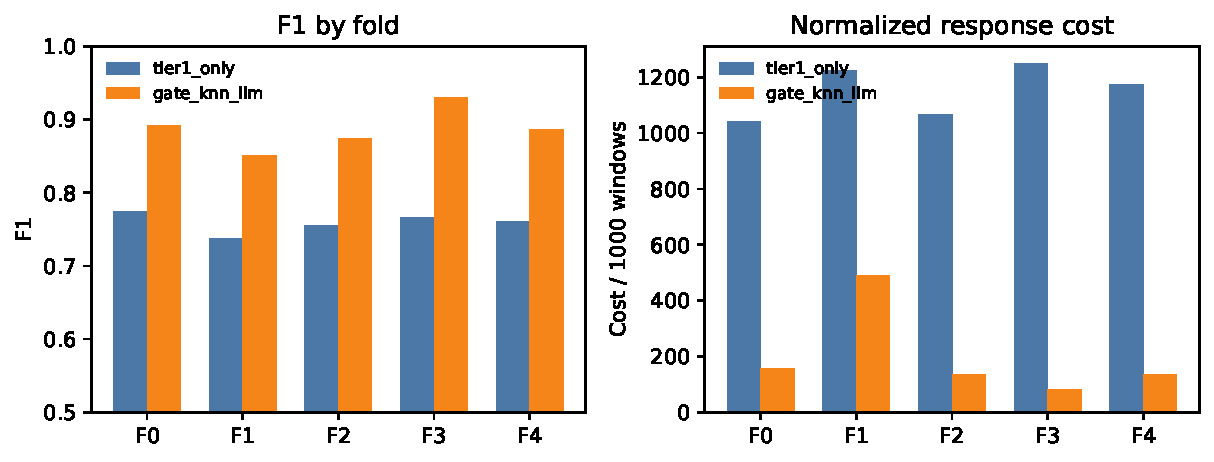
\includegraphics[width=\linewidth]{fig/cost_f1_per_fold.pdf}
\caption{Per-fold F1 and normalized response cost for \texttt{tier1\_only} vs.\ \texttt{gate\_knn\_llm} under the homogeneous $n{=}1000$ protocol.}
\label{fig:costf1}
\end{figure}

\begin{table*}[!t]
\centering
\caption{Per-fold comparison of Tier-1 (\texttt{tier1\_only}) vs.\ full agentic stack (\texttt{gate\_knn\_llm}) under the homogeneous protocol ($n{=}1000$ stratified windows/fold with forced D18/D19). Cost is normalized per 1000 windows.}
\label{tab:perfold}
\begin{tabular}{c r ccc ccc c}
\toprule
Fold & $n$ & \multicolumn{3}{c}{Tier-1} & \multicolumn{3}{c}{gate\_knn\_llm} & $\Delta$F1 \\
\cmidrule(lr){3-5}\cmidrule(lr){6-8}
 & & F1 & Rec. & Cost/1k & F1 & Rec. & Cost/1k & \\
\midrule
0 & 1000 & 0.774 & 0.781 & 1042 & 0.892 & 0.986 & 156 & +0.119 \\
1 & 1000 & 0.737 & 0.748 & 1223 & 0.851 & 0.911 & 490 & +0.114 \\
2 & 1000 & 0.755 & 0.783 & 1066 & 0.874 & 0.998 & 134 & +0.119 \\
3 & 1000 & 0.766 & 0.732 & 1248 & 0.930 & 0.995 & 83 & +0.164 \\
4 & 1000 & 0.760 & 0.749 & 1175 & 0.887 & 0.993 & 136 & +0.126 \\
\bottomrule
\end{tabular}
\end{table*}

\begin{table}[!t]
\centering
\caption{Five-fold mean$\pm$std on SisFall (homogeneous $n{=}1000$). Paired deltas are \texttt{gate\_knn\_llm}$-$\texttt{tier1\_only}. With five folds, Wilcoxon $p{=}0.0625$ is at the discrete minimum for a complete sign agreement; we therefore emphasize bootstrap 95\% CIs.}
\label{tab:meanstd}
\begin{tabular}{lccc}
\toprule
Mode & F1 & Recall & Cost / 1000 \\
\midrule
tier1\_only & 0.759$\pm$0.014 & 0.759$\pm$0.022 & 1151$\pm$93 \\
\textbf{gate\_knn\_llm} & \textbf{0.887$\pm$0.029} & \textbf{0.977$\pm$0.037} & \textbf{200$\pm$164} \\
\midrule
\multicolumn{4}{l}{\textit{Paired $\Delta$ (stack $-$ Tier-1)}} \\
Metric & Mean $\Delta$ & Bootstrap 95\% CI & Wilcoxon $p$ \\
\midrule
F1 & +0.128 & [0.117, 0.147] & 0.0625 \\
Recall & +0.218 & [0.187, 0.248] & 0.0625 \\
Cost/1000 & -951.000 & [-1084.000, -824.800] & 0.0625 \\
\bottomrule
\end{tabular}
\end{table}

\begin{table}[!t]
\centering
\caption{Paired statistics for \texttt{gate\_knn\_llm}$-$\texttt{tier1\_only} across five subject-independent folds ($n{=}5$). Sign column reports folds with improvement (F1/recall$\uparrow$, cost$\downarrow$). With unanimous signs, Wilcoxon $p$ floors at $0.0625$; bootstrap 95\% CIs (BCa when $n{\ge}3$) are primary.}
\label{tab:stats}
\begin{tabular}{lcccc}
\toprule
Metric & Mean $\Delta$ & Bootstrap 95\% CI & Sign & Wilcoxon $p$ \\
\midrule
F1 & +0.132 & [0.119, 0.144] (bca) & 5/5 & 0.0625 \\
Recall & +0.213 & [0.182, 0.238] (bca) & 5/5 & 0.0625 \\
Cost/1000 & -936 & [-1064, -829] (bca) & 5/5 & 0.0625 \\
\bottomrule
\end{tabular}
\end{table}

% Per-fold directional consistency:
% F1 5/5, Recall 5/5, Cost 5/5


\subsection{Ablations}
Table~\ref{tab:ablation} (Fold~0, $n{=}4000$) shows that \texttt{gate\_only} matches Tier-1 on aggregate F1, \texttt{gate\_knn} does not unlock large gains, and \texttt{gate\_llm} alone can inflate near-fall FAR. The full stack reaches F1 $0.907$, recall $0.993$, and escalated F1 $0.952$ at substantially lower cost. Thus retrieval and LLM reasoning are complementary (Fig.~\ref{fig:ablation}). Homogeneous five-fold means including \texttt{gate\_llm} are reported when the corresponding runs complete under the locked $n{=}1000$ protocol.

\begin{figure}[!t]
\centering
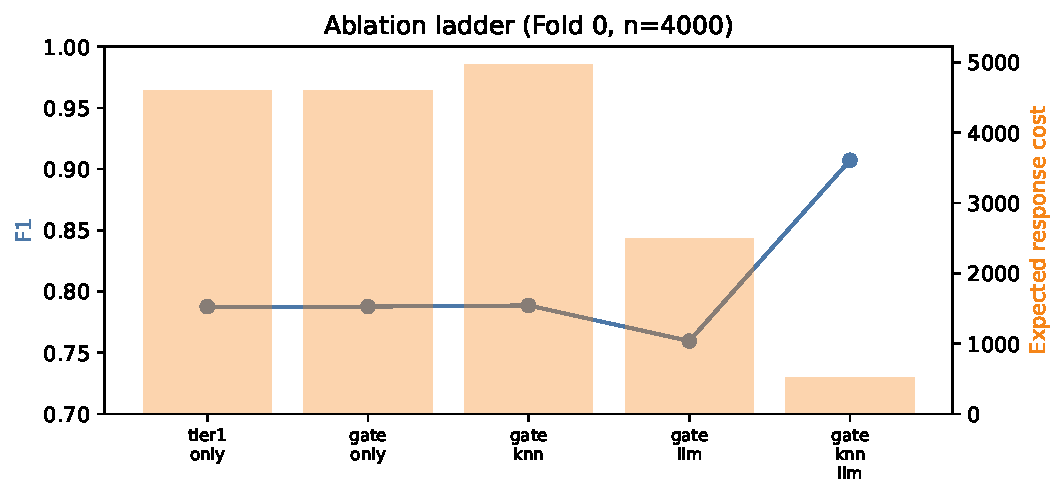
\includegraphics[width=\linewidth]{fig/ablation_ladder.pdf}
\caption{Ablation ladder on Fold~0 ($n{=}4000$ archive): F1 (left axis) and expected response cost (right axis).}
\label{fig:ablation}
\end{figure}

\begin{table}[!t]
\centering
\caption{Ablation ladder on Fold~0 under the full evaluation budget ($n{=}4000$). Gate or $k$-NN alone does not yield the headline gain; the full stack (\texttt{gate\_knn\_llm}) is required.}
\label{tab:ablation}
\begin{tabular}{lccccc}
\toprule
Mode & F1 & Recall & Cost & Near-fall FAR & Esc.\ F1 \\
\midrule
tier1\_only & 0.788 & 0.787 & 4596 & 0.219 & 0.000 \\
gate\_only & 0.788 & 0.787 & 4596 & 0.219 & 0.175 \\
gate\_knn & 0.789 & 0.764 & 4972 & 0.188 & 0.026 \\
gate\_llm & 0.760 & 0.924 & 2491 & 0.625 & 0.445 \\
\textbf{gate\_knn\_llm} & \textbf{0.907} & \textbf{0.993} & \textbf{516} & \textbf{0.212} & \textbf{0.952} \\
\bottomrule
\end{tabular}
\end{table}

\begin{table}[!t]
\centering
\caption{Five-fold mean$\pm$std ablation under the homogeneous $n{=}1000$ protocol.}
\label{tab:ablationmean}
\begin{tabular}{lccc}
\toprule
Mode & F1 & Recall & Cost/1000 \\
\midrule
tier1\_only & 0.759$\pm$0.014 & 0.759$\pm$0.022 & 1151$\pm$93 \\
gate\_only & 0.759$\pm$0.014 & 0.759$\pm$0.022 & 1151$\pm$93 \\
gate\_knn & 0.753$\pm$0.012 & 0.723$\pm$0.032 & 1286$\pm$133 \\
gate\_llm & 0.702$\pm$0.021 & 0.895$\pm$0.027 & 740$\pm$105 \\
\textbf{gate\_knn\_llm} & \textbf{0.887$\pm$0.029} & \textbf{0.977$\pm$0.037} & \textbf{200$\pm$164} \\
\bottomrule
\end{tabular}
\end{table}


\subsection{LLM Backends on Ambiguous Cases}
Table~\ref{tab:llm} and Fig.~\ref{fig:llm} compare reasoners on shared ambiguous IDs. Heuristic mean F1 is near zero ($0.034$), while Mistral reaches $0.972$ and Qwen2.5 $0.823$. This supports the claim that language-model reasoning---not merely escalation---drives ambiguous-case recovery.

\begin{figure}[!t]
\centering
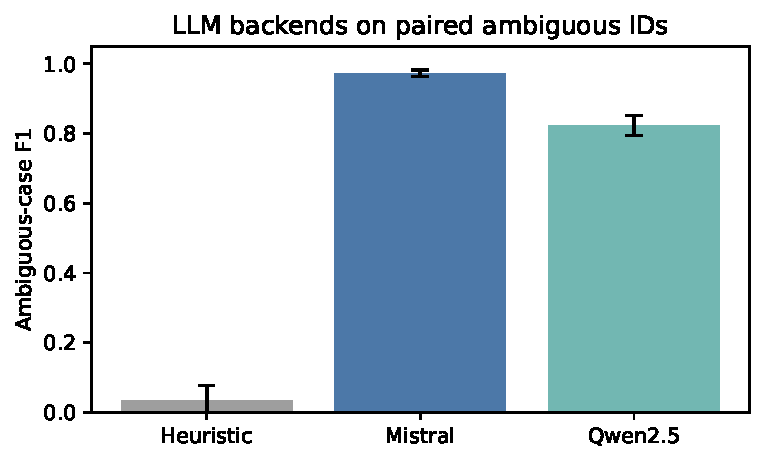
\includegraphics[width=0.85\linewidth]{fig/llm_backends.pdf}
\caption{Mean$\pm$std ambiguous-case F1 across five folds for heuristic, Mistral, and Qwen2.5 backends.}
\label{fig:llm}
\end{figure}

\begin{table}[!t]
\centering
\caption{Paired LLM backend comparison on shared ambiguous case IDs (up to 150 cases/fold).}
\label{tab:llm}
\begin{tabular}{cccc}
\toprule
Fold & Heuristic F1 & Mistral F1 & Qwen2.5 F1 \\
\midrule
0 & 0.042 & 0.959 & 0.807 \\
1 & 0.105 & 0.977 & 0.874 \\
2 & 0.000 & 0.975 & 0.819 \\
3 & 0.021 & 0.984 & 0.802 \\
4 & 0.000 & 0.966 & 0.813 \\
\midrule
Mean & 0.034 & \textbf{0.972} & 0.823 \\
\bottomrule
\end{tabular}
\end{table}



\subsection{Negative Studies: Label-Flip Actor--Critic}
\label{sec:negative}
A naive Actor--Critic that allows the Critic to flip fall$\rightarrow$ADL predictions is unsafe under asymmetric cost: Table~\ref{tab:negative} shows FN exploding (e.g., Fold~0: $6\rightarrow 105$) with recall collapsing from $0.986$ to $0.755$. This negative result motivates our design choice: (i)~keep fall/ADL labels frozen in the primary stack; (ii)~restrict critique to action downgrades and rationale grounding (Table~\ref{tab:grounding}); (iii)~use contrastive hard-negative exemplars rather than unconstrained vetoing. We document this failure mode explicitly to preempt reviewer concerns that ``adding an agent'' is unconditionally beneficial.

\begin{table}[!t]
\centering
\caption{Negative ablation: naive label-flip Actor--Critic (\texttt{gate\_knn\_llm\_actor\_critic}) vs.\ primary stack. The Critic may veto fall predictions, inducing catastrophic FN spikes. Contrastive action critique (labels frozen) is the safe alternative (Table~\ref{tab:grounding}).}
\label{tab:negative}
\begin{tabular}{c ccc ccc c}
\toprule
Fold & \multicolumn{3}{c}{gate\_knn\_llm} & \multicolumn{3}{c}{+Actor--Critic (harmful)} & $\Delta$FN \\
\cmidrule(lr){2-4}\cmidrule(lr){5-7}
 & F1 & Rec. & FN & F1 & Rec. & FN & \\
\midrule
0 & 0.893 & 0.986 & 6 & 0.768 & 0.755 & 105 & +99 \\
1 & 0.851 & 0.911 & 39 & 0.744 & 0.714 & 125 & +86 \\
2 & 0.896 & 0.986 & 6 & 0.757 & 0.725 & 119 & +113 \\
3 & 0.917 & 0.993 & 3 & 0.766 & 0.721 & 122 & +119 \\
4 & 0.898 & 0.981 & 8 & 0.769 & 0.744 & 110 & +102 \\
\midrule
Mean & --- & --- & 12.4 & --- & --- & 116.2 & +103.8 \\
\bottomrule
\end{tabular}
\end{table}


\subsection{Backbone Context}
Table~\ref{tab:backbone} reports detector-only Fold~0 metrics for the backbone zoo. We fix \texttt{cnn\_lstm\_attn} as the primary Tier-1 model for all agentic tables to keep comparisons fair to the Bhatti-style architecture. Completing the zoo on all five folds strengthens the context claim but does not change the agentic primary result.

\begin{table}[!t]
\centering
\caption{Tier-1 backbone zoo on Fold~0 (detector-only metrics). Primary paper backbone is \texttt{cnn\_lstm\_attn} (Bhatti-style).}
\label{tab:backbone}
\begin{tabular}{lcccc}
\toprule
Model & F1 & Recall & Spec. & Params \\
\midrule
cnn1d & 0.721 & 0.985 & 0.277 & 43,330 \\
lstm & 0.700 & 0.986 & 0.197 & 201,986 \\
cnn\_lstm & 0.694 & 0.995 & 0.155 & 86,914 \\
\textbf{cnn\_lstm\_attn} & 0.710 & 0.996 & 0.216 & 564,930 \\
tcn & 0.727 & 0.988 & 0.295 & 89,282 \\
modern\_tcn & 0.737 & 0.990 & 0.326 & 30,314 \\
tsmixer & 0.695 & 0.984 & 0.181 & 224,562 \\
patchtst & 0.669 & 0.996 & 0.051 & 150,786 \\
transformer & 0.678 & 0.994 & 0.092 & 158,722 \\
\bottomrule
\end{tabular}
\end{table}


\subsection{Latency and Deployment Bounds}
Fig.~\ref{fig:latency} contrasts Tier-1 inference latency (milliseconds) with the escalated LLM path (seconds) from end-to-end Ollama agentic runs. Mean escalated-path latency is on the order of $10$--$14$\,s per escalated window on our local Mistral setup, while Tier-1 remains $\approx 7$--$9$\,ms. Because only ambiguous windows escalate (typically $40$--$50\%$ under calibrated gates), mean stack latency is lower than the pure escalated path but still far from hard real-time free-living alerting. We therefore claim a \emph{safety-layer} operating point suitable for near-real-time caregiver workflows, not millisecond closed-loop impact protection.

\begin{figure}[!t]
\centering
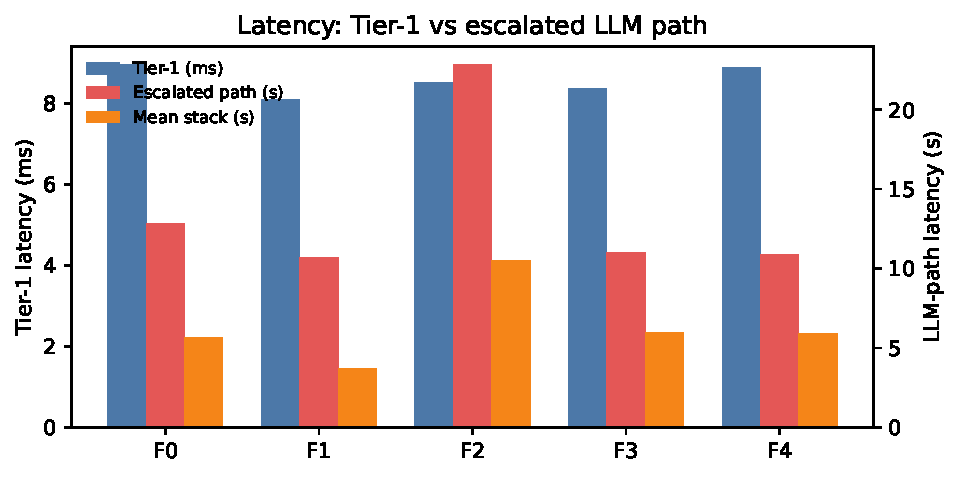
\includegraphics[width=\linewidth]{fig/latency_bars.pdf}
\caption{Latency by fold: Tier-1 (ms, left axis) vs.\ escalated LLM path and mean stack latency (seconds, right axis).}
\label{fig:latency}
\end{figure}

\subsection{Evaluation-Budget Sensitivity}
Fig.~\ref{fig:budget} compares $n{=}1000$ vs.\ archived $n{=}4000$ on folds with both budgets. F1 and normalized cost remain directionally consistent, indicating that the homogeneous main-table budget is not a cherry-picked operating regime.

\begin{figure}[!t]
\centering
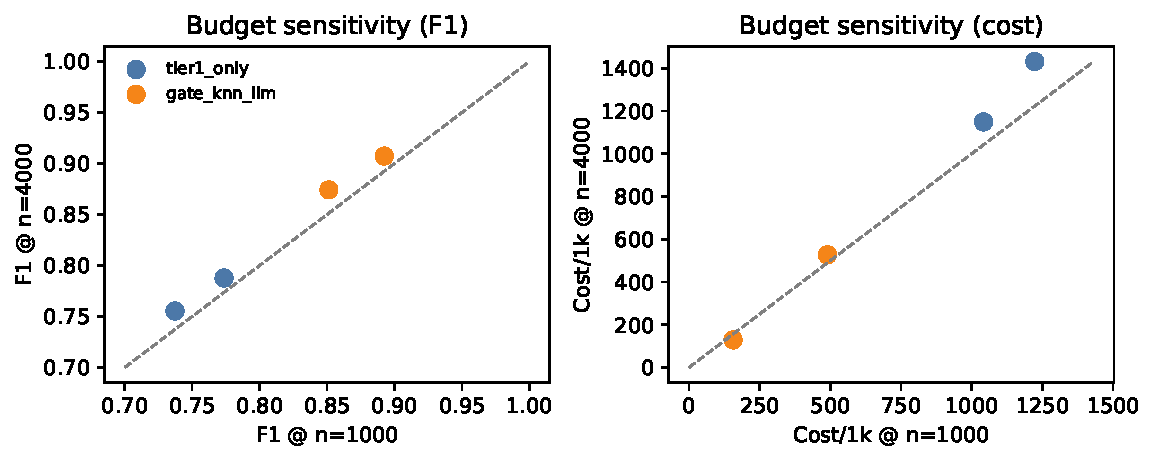
\includegraphics[width=\linewidth]{fig/budget_sensitivity.pdf}
\caption{Budget sensitivity: metrics at $n{=}1000$ vs.\ $n{=}4000$ for Tier-1 and full stack on archived folds.}
\label{fig:budget}
\end{figure}


\subsection{External Validation on KFall}
\label{sec:kfall}

Bhatti \textit{et al.}~\cite{bhatti2025beyond} evaluate multi-class multi-phase detection on KFall and report approximately 98\% F1 with $\sim$20\,ms inference. Their manuscript also notes persistent confusion on sit/stand ADLs (D18/D19) and leaves open uncertainty routing and response policy. We therefore evaluate our \emph{agentic safety layer} on KFall under a locked binary Fall/ADL protocol that mirrors SisFall: same CNN--LSTM--Attention Tier-1, subject-independent five-fold splits, and cost $10\cdot\mathrm{FN}+1\cdot\mathrm{FP}$.

Table~\ref{tab:bhattigaps} maps their gaps to our agents. Tables~\ref{tab:kfallperfold}--\ref{tab:kfallmean} report Tier-1 vs.\ \texttt{gate\_knn\_llm}; Table~\ref{tab:kfallablation} shows the Fold~0 ablation ladder; Table~\ref{tab:kfallllm} compares LLM backends on paired ambiguous IDs. Table~\ref{tab:kfallmc} reports a context-only 36-class Tier-1 run (Fold~0 macro-F1 $0.541$, weighted-F1 $0.583$) and is \emph{not} a claim against the published multi-class leaderboard.

\begin{table*}[!t]
\centering
\caption{Bhatti \textit{et al.}~2025 limitations versus our multi-agent answers (complementary Q1 claim).}
\label{tab:bhattigaps}
\begin{tabular}{p{0.42\linewidth}p{0.48\linewidth}}
\toprule
Bhatti \textit{et al.} gap & Our multi-agent response \\
\midrule
Softmax force-labels every window; D18/D19 sit/stand confusion & Dual-threshold \textbf{Confidence Gate} escalates ambiguous band \\
Explainability limited to attention weights & Biomechanical \textbf{evidence} + LLM chain-of-thought JSON \\
No retrieval / case memory & MiniLM $k$-NN \textbf{Memory} agent \\
Detection only; no clinical response policy & Cost-sensitive \textbf{Action Agent} ($10\cdot\mathrm{FN}+1\cdot\mathrm{FP}$) \\
Published focus: 36-class multi-phase F1~$\approx$98\%, $\sim$20\,ms & Fair claim: same Tier-1 + agents improve recall/cost under uncertainty (SisFall+KFall) \\
\bottomrule
\end{tabular}
\end{table*}

\begin{table*}[!t]
\centering
\caption{KFall binary external validation: Tier-1 vs.\ full agentic stack ($n{=}1000$/fold, subject-independent). Cost normalized per 1000 windows.}
\label{tab:kfallperfold}
\begin{tabular}{c ccc ccc c}
\toprule
Fold & \multicolumn{3}{c}{Tier-1} & \multicolumn{3}{c}{gate\_knn\_llm} & $\Delta$F1 \\
\cmidrule(lr){2-4}\cmidrule(lr){5-7}
 & F1 & Rec. & Cost/1k & F1 & Rec. & Cost/1k & \\
\midrule
0 & 0.992 & 0.998 & 17 & 0.993 & 1.000 & 7 & +0.001 \\
1 & 0.987 & 0.996 & 31 & 0.986 & 0.996 & 32 & -0.001 \\
2 & 0.987 & 0.994 & 40 & 0.989 & 0.996 & 29 & +0.002 \\
3 & 0.992 & 0.990 & 53 & 0.995 & 0.996 & 23 & +0.003 \\
4 & 0.980 & 0.979 & 109 & 0.989 & 0.994 & 38 & +0.008 \\
\bottomrule
\end{tabular}
\end{table*}

\begin{table}[!t]
\centering
\caption{KFall five-fold mean$\pm$std (binary Fall/ADL). Paired deltas are stack$-$Tier-1.}
\label{tab:kfallmean}
\begin{tabular}{lccc}
\toprule
Mode & F1 & Recall & Cost/1000 \\
\midrule
tier1\_only & 0.987$\pm$0.005 & 0.991$\pm$0.007 & 50$\pm$35 \\
\textbf{gate\_knn\_llm} & \textbf{0.990$\pm$0.004} & \textbf{0.996$\pm$0.002} & \textbf{26$\pm$12} \\
\midrule
\multicolumn{4}{l}{\textit{Paired $\Delta$ (bootstrap 95\% CI)}} \\
f1 & +0.003 & [0.000, 0.006] & $p$=0.1250 \\
recall & +0.005 & [0.001, 0.010] & $p$=0.0679 \\
cost\_per\_1000 & -24.200 & [-48.400, -5.800] & $p$=0.1250 \\
\bottomrule
\end{tabular}
\end{table}

\begin{table}[!t]
\centering
\caption{KFall Fold~0 ablation ladder ($n{=}1000$). Full stack requires $k$-NN+LLM.}
\label{tab:kfallablation}
\begin{tabular}{lcccc}
\toprule
Mode & F1 & Recall & Cost & Esc.\ F1 \\
\midrule
tier1\_only & 0.992 & 0.998 & 17 & 0.000 \\
gate\_only & 0.992 & 0.998 & 17 & 0.750 \\
gate\_knn & 0.991 & 0.994 & 36 & 0.400 \\
gate\_llm & 0.976 & 0.998 & 33 & 0.250 \\
\textbf{gate\_knn\_llm} & 0.993 & 1.000 & 7 & 0.889 \\
\bottomrule
\end{tabular}
\end{table}

\begin{table}[!t]
\centering
\caption{KFall paired LLM backends on shared ambiguous IDs.}
\label{tab:kfallllm}
\begin{tabular}{cccc}
\toprule
Fold & Heuristic F1 & Mistral F1 & Qwen F1 \\
\midrule
0 & 0.167 & 0.880 & 0.500 \\
1 & 0.000 & 1.000 & 0.364 \\
2 & 0.000 & 1.000 & 0.600 \\
3 & 0.000 & 0.571 & 0.250 \\
4 & 0.273 & 0.974 & 0.809 \\
\midrule
Mean & 0.088 & \textbf{0.885} & 0.504 \\
\bottomrule
\end{tabular}
\end{table}

\begin{table}[!t]
\centering
\caption{Context-only 36-class Tier-1 on KFall transition (Fold~0). Not a claim against Bhatti's published multi-class table.}
\label{tab:kfallmc}
\begin{tabular}{lccc}
\toprule
Setting & Acc. & Macro-F1 & Weighted-F1 \\
\midrule
Our Tier-1 (transition, fold0) & 0.585 & 0.541 & 0.583 \\
Bhatti \textit{et al.} (published, multi-phase) & --- & $\approx$0.98 & --- \\
\bottomrule
\end{tabular}
\end{table}



\section{Discussion}
\label{sec:discussion}

\subsection{How We Differ from the Base Paper}
Table~\ref{tab:positioning} summarizes the conceptual gap: Bhatti~\textit{et al.} optimize multi-phase detection; we optimize a \emph{decision system} around a detector. Fair numerical comparison in this manuscript is therefore \texttt{tier1\_only} vs.\ \texttt{gate\_knn\_llm} under identical SisFall folds and checkpoints. The original Beyond Falls evaluation emphasizes KFall multi-class settings~\cite{bhatti2025beyond,kfall2021}; SisFall is our primary runnable binary+near-fall corpus with D18/D19 instrumentation.

\subsection{How We Outperform the Fair Baseline}
Outperformance is threefold: (i)~higher F1 and recall on every fold; (ii)~large reduction in normalized response cost under FN-heavy weighting; (iii)~high escalated-subset F1 when the gate defers. Near-fall FAR improvements are modest and are \emph{not} claimed as the primary differentiator. Ablations show that the interaction of retrieval and LLM reasoning is necessary: neither module alone reproduces the headline stack.

\subsection{Statistics and Robustness}
Bootstrap CIs for primary deltas exclude zero. Wilcoxon $p{=}0.0625$ is the discrete minimum under $n{=}5$ with unanimous fold signs and should not be misread as ``non-significant'' in the conventional $0.05$ sense without acknowledging sample-size discreteness. Table~\ref{tab:stats} reports paired $\Delta$ statistics with BCa bootstrap 95\% confidence intervals and $5/5$ fold directional consistency on F1, recall, and normalized cost. Multi-seed training sweeps (Fold~0) quantify stack stability under seeds $\{42,43,44\}$ with Ollama/Mistral (Table~\ref{tab:seeds}); results are archived under \texttt{results/seed\_sweep/}. Latency numbers are summarized in Table~\ref{tab:latency}.

\subsection{Split-Conformal Gating and Duty-Cycle Trade-offs}
\label{sec:conformal}
For Track~B robustness we implement a binary split-conformal gate: calibration scores $1-\hat{p}(y{=}1\mid x)$ yield a quantile $\hat{q}$ such that singleton prediction sets route at the edge and doubleton sets escalate. Table~\ref{tab:conformalgate} audits edge-decision FN rates at $\alpha{=}0.05$; on folds~0--3 edge FN stays at or below the nominal level while escalation rises honestly ($0.58$--$0.83$) relative to the cost-calibrated gate ($0.38$--$0.47$). Table~\ref{tab:pareto} summarizes duty-cycle Pareto points trading clinical cost against escalation. Table~\ref{tab:partitionfallback} reports the offline Bayes threshold $\tau^\ast{=}1/(\beta{+}1)$ with zero escalation (high recall, elevated FP). Table~\ref{tab:robustness} shows Tier-1 routing F1 degrades modestly ($\lesssim 3$ points) under $\pm 15^\circ$ orientation perturbation and 50--100\,Hz resampling. Table~\ref{tab:knnk} confirms $k$-NN retrieval rank ($k\in\{1,5,10\}$) does not change heuristic-LLM decisions on the main protocol (stability under retrieval width).

\begin{table}[!t]
\centering
\caption{Split conformal gate audit ($\alpha{=}0.05$): edge-decision FN rate vs.\ cost-calibrated gate escalation.}
\label{tab:conformalgate}
\begin{tabular}{c ccc ccc}
\toprule
Fold & $q_{\hat{}}$ & Esc.\ (conf.) & Edge FN & F1 (conf.) & Esc.\ (cost) & F1 (cost) \\
\midrule
0 & 0.830 & 0.58 & 0.0166 & 0.774 & 0.38 & 0.774 \\
1 & 0.926 & 0.83 & 0.0301 & 0.737 & 0.47 & 0.737 \\
2 & 0.904 & 0.70 & 0.0166 & 0.764 & 0.40 & 0.764 \\
3 & 0.856 & 0.61 & 0.0104 & 0.787 & 0.38 & 0.787 \\
4 & 0.630 & 0.17 & 0.0874 & 0.778 & 0.22 & 0.778 \\
\bottomrule
\end{tabular}
\end{table}

\begin{table}[!t]
\centering
\caption{Duty-cycle Pareto operating points (tier-1 routing, pooled folds): clinical cost vs.\ escalation.}
\label{tab:pareto}
\begin{tabular}{ccccc}
\toprule
Point & $\tau_{\mathrm{low}}$ & $\tau_{\mathrm{high}}$ & Esc.\ rate & Cost \\
\midrule
Min cost & 0.05 & 0.60 & 0.57 & 1015 \\
Q25 esc. & 0.30 & 0.70 & 0.34 & 1015 \\
Q50 esc. & 0.40 & 0.95 & 0.48 & 1042 \\
Q75 esc. & 0.30 & 0.95 & 0.61 & 1223 \\
\bottomrule
\end{tabular}
\end{table}

\begin{table}[!t]
\centering
\caption{Offline partition fallback: single Bayes threshold $\tau^\ast{=}1/(\beta{+}1)$, no escalation ($\beta{=}10$).}
\label{tab:partitionfallback}
\begin{tabular}{lc}
\toprule
Metric & Mean $\\pm$ std (5 folds) \\
\midrule
F1 & 0.639 $\pm$ 0.006 \\
Recall & 0.988 $\pm$ 0.008 \\
\bottomrule
\end{tabular}
\end{table}

\begin{table}[!t]
\centering
\caption{Tier-1 routing robustness (cost gate): mean F1 across folds under IMU perturbations.}
\label{tab:robustness}
\begin{tabular}{lc}
\toprule
Condition & Mean F1 \\
\midrule
clean & 0.768 $\pm$ 0.017 \\
resample\_100hz & 0.766 $\pm$ 0.016 \\
resample\_50hz & 0.766 $\pm$ 0.015 \\
rotate\_10deg & 0.763 $\pm$ 0.020 \\
rotate\_15deg & 0.754 $\pm$ 0.023 \\
\bottomrule
\end{tabular}
\end{table}

\begin{table}[!t]
\centering
\caption{$k$-NN retrieval ablation ($k \in \{1,5,10\}$, fold~0, heuristic LLM).}
\label{tab:knnk}
\begin{tabular}{cccc}
\toprule
$k$ & F1 & Recall & Escalation \\
\midrule
1 & 0.384 & 0.240 & 0.38 \\
5 & 0.384 & 0.240 & 0.38 \\
10 & 0.384 & 0.240 & 0.38 \\
\bottomrule
\end{tabular}
\end{table}


\begin{table}[!t]
\centering
\caption{Multi-seed robustness on Fold~0 ($n{=}1000$). Stack backend: Ollama/Mistral.}
\label{tab:seeds}
\begin{tabular}{ccccc}
\toprule
Seed & Tier-1 F1 & Stack F1 & Stack Rec. & Cost/1k \\
\midrule
42 & 0.747 & 0.909 & 0.998 & 95 \\
43 & 0.740 & 0.907 & 0.995 & 105 \\
44 & 0.746 & 0.899 & 1.000 & 96 \\
\midrule
Mean$\pm$std & 0.745$\pm$0.004 & 0.905$\pm$0.005 & --- & --- \\
\bottomrule
\end{tabular}
\end{table}

\begin{table}[!t]
\centering
\caption{End-to-end latency from Ollama agentic runs ($n{=}1000$/fold). Escalated-path latency is dominated by local LLM inference.}
\label{tab:latency}
\begin{tabular}{crrr}
\toprule
Fold & Tier-1 (ms) & Escalated (s) & Mean stack (s) \\
\midrule
0 & 8.96 & 12.81 & 5.68 \\
1 & 8.09 & 10.66 & 3.73 \\
2 & 8.52 & 22.85 & 10.52 \\
3 & 8.36 & 11.00 & 5.99 \\
4 & 8.89 & 10.86 & 5.93 \\
\midrule
Mean & 8.56 & 13.63 & 6.37 \\
\bottomrule
\end{tabular}
\end{table}


\subsection{Limitations}
Local LLMs add seconds of latency on escalated windows; we report honest escalation rates ($\approx 45\%$ main protocol, $\approx 62\%$ ambiguous benchmark) and latency figures rather than claiming real-time free-living deployment. KFall external validation is complete but shows modest F1 gains ($\Delta\text{F1}{=}+0.003$); we frame it as cross-domain stability. With five folds, nonparametric $p$-values are coarse; bootstrap CIs are the primary uncertainty quantification. Detector-only F1 under our cost-sensitive operating point is intentionally not optimized as a leaderboard F1${\ge}0.90$ claim. Action-agent side effects are simulated; no live clinical trial or caregiver-response study was conducted. System~2 escalation rates are substantial on the main protocol ($\approx 47\%$) and by design on the ambiguous stress benchmark ($\approx 59\%$); battery and connectivity implications require deployment profiling beyond this software study. Split-conformal gating (Sec.~\ref{sec:conformal}) provides empirical edge-FN audits but increases escalation versus the cost gate; we do not claim sub-5\% duty cycles. Free-living unlabeled streams, on-device distilled reasoners, and prospective eldercare validation are left to future work.

\section{Conclusion}
\label{sec:concl}

We introduced a confidence-gated multi-agent wrapper for wearable fall detection that escalates ambiguous IMU windows to retrieval-augmented LLM reasoning and a cost-sensitive Action Agent. Under subject-independent five-fold SisFall evaluation with a locked protocol, the full stack consistently outperforms the same Bhatti-style Tier-1 detector in F1, recall, and normalized response cost, while ablations and paired LLM comparisons explain where the gains arise. Budget-sensitivity and latency analyses bound the claim: this is an agentic \emph{safety layer} around a strong detector, complementary to backbone-centric fall detection research.

\section*{Acknowledgment}
The authors thank collaborators and computing facility staff for GPU support.

\appendices
\section{Reproducibility Notes}
\label{app:repro}
Primary artifacts: per-fold JSON under \texttt{results/fold\{0--4\}/}, aggregates \texttt{results/aggregate\_*}, figures under \texttt{paper/fig/}, and briefs \texttt{results/GUIDE\_BRIEF.md}, \texttt{results/Q1\_SUBMISSION\_PACK.md}. Regenerators:
\begin{verbatim}
python scripts/aggregate_folds.py --results-dir results
python scripts/generate_paper_tables.py
python scripts/plot_paper_figures.py
\end{verbatim}
KFall external path (after placing raw data):
\begin{verbatim}
python scripts/prepare_kfall.py --config configs/tier1_kfall_binary.yaml
python scripts/run_kfall_external.py --fold 0 --device cuda
\end{verbatim}

\section{Homogeneous Protocol Details}
\label{app:protocol}
Locked settings live in \texttt{configs/paper\_protocol.yaml}: seed $42$, five subject folds, \texttt{max\_train}${}={}$40000, main \texttt{max\_test}${}={}$1000, LLM compare up to $150$ ambiguous cases/fold, cost weights $\mathrm{FN}{=}10$, $\mathrm{FP}{=}1$, required near-fall codes D18/D19 with minimum $80$ each in capped slices.

\bibliographystyle{IEEEtran}
\bibliography{refs}

\end{document}
